\documentclass[10pt,a4paper]{scrartcl}
\pagestyle{empty}
\usepackage{a4} % alternativ \usepackage{a4wide}
\usepackage[ngerman]{babel} % Neudeutsche Silbentrennung (mehrsprachiges Dokument)
\usepackage{parskip} % Skip indentation of first row
\usepackage{graphicx} % Graphics support
\usepackage{longtable} % Tables across several pages
\usepackage{hyperref} % Hyperlinks
\usepackage[automark]{scrpage2} %kopf/fusszeile
\usepackage[utf8x]{inputenc} % Unicode-Encoding
 
\linespread{1.3}

\author{Danilo Bargen, Christian Fässler, Jonas Furrer} 
\title{Anforderungsspezifikation\\ Projekt BierIdee}

\pagestyle{scrheadings}
\ihead{SE2 Projekte} %linke Kopfzeile
\ohead{BierIdee} %rechte Kopfzeile

\begin{document}

\begin{titlepage}
	\maketitle
	\vspace{120mm}
	\thispagestyle{empty} % Don't start page numbers on this page
\end{titlepage}


\section{Einführung}
\subsection{Zweck}
Dieses Dokument zeigt die Resultate der Elaborationphase, in der die Anforderungen an das Produkt erfasst wurden.
\subsection{Gültigkeitsbereich}
Die Gültigkeit des Dokumentes beschränkt sich auf die Dauer des SE2-Projekte Modules FS2012.
\subsection{Definitionen und Abkürzungen}
Die Definitionen und Abkürzungen befinden sich im Dokument Glossary.
\subsection{Referenzen}
\begin{itemize}
\item Glossary.BierIdee.pdf
\item Usecases.fully.dressed.format.pdf
\item Projektantrag.pdf
\item Supplementary.specification.pdf
\end{itemize}

\subsection{Übersicht}
In diesem Dokument werden die Anforderungen an das Projekt BierIdee ausgearbeitet und festgehalten. Grundsätzlich beinhalten sie die Resultate der Elaborationphase des Projektes. Das Dokument besteht im Groben aus zwei Teilen: Den funktionalen und nicht funktionalen Anforderungen. Als Anhaltspunkt für die nicht funktionalen Anforderungen gilt der FURPS+ Standard.
\newpage

\section{Allgemeine Beschreibung}
\subsection{Produktperspektive}
Die Perspektive dieses Produktes wurde im Projektantrag festgehalten.

\subsection{Produkt Funktion}
Die Hauptfunktion des zu entwickelnden Systemes ist es, ein Portal zu bieten welches das Erfassen und bewerten von Bieren ermöglicht. Anhand von persönlichen "Aktivitäten" werden individuelle Empfehlungen für Biersorten erstellt. Da sich das Projekt sehr gut mit Features erweitern lässt, wurden die identifizierten Möglichkeiten in zwei Kategorien aufgeteilt. Für dieses Projekt stehen die primären Features im Fokus. Falls es die Zeit zulässt, kann das System problemlos um weitere Features erweitert werden.

\subsubsection{Primäre Features}
\begin{itemize}
\item Verzeichnis mit Biersorten und Brauereien
\item Benutzerkonten/Profile
\item Erfassen/Bearbeiten von Bieren durch Benutzer
\item Taggen von Bieren mit Attributen wie bspw. Sorte
\item Bewerten von Biersorten durch Benutzer
\item Individuelle Bier-Empfehlungen
\item Erfassung von Benutzer-Aktivitäten (z. B Bierkonsum)
\item Timeline mit Aktivitäten
\item Internationalisierung 
\end{itemize}

\subsubsection{Erweiterungemöglichkeiten}
\begin{itemize}
\item Location-Based Services
\item Achievements/Badges für bestimmte Benutzeraktivitäten
\item Biere mit Barcode erfassen
\item Fotos von Bieren hochladen
\item Offizielle Brauereiprofile
\item Barprofile
\item Checkin in Bars
\item Bierquiz
\item Statistiken (z. B. Top rated, most consumed etc.)
\item Integration in bestehende Social-Networks
\end{itemize}

\subsection{Benutzer Charakteristik}
Zum Zielpublikum gehören Power-User von Android Geräten welche häufig Soziale Netzwerke benutzen und gelegentlich ein Bier trinken. Es wird davon ausgegangen, dass es sich auch im technischen Sinne um Fortgeschrittene Benutzer handelt, welche bereits einige Erfahrung mit der Bedienung von Android Applikationen haben.
\subsection{Einschränkungen}
Das System beschränkt sich clientseitig auf Androidgeräte mit dem API Level 10. Weitere Angaben im Kapitel nicht funktionale Anforderungen.
\subsection{Annahmen}
Für das Projekt wurden keine Annahmen getroffen.

\section{Funktionale Anforderungen / Use Cases}
\subsection{Use Case Diagramm}
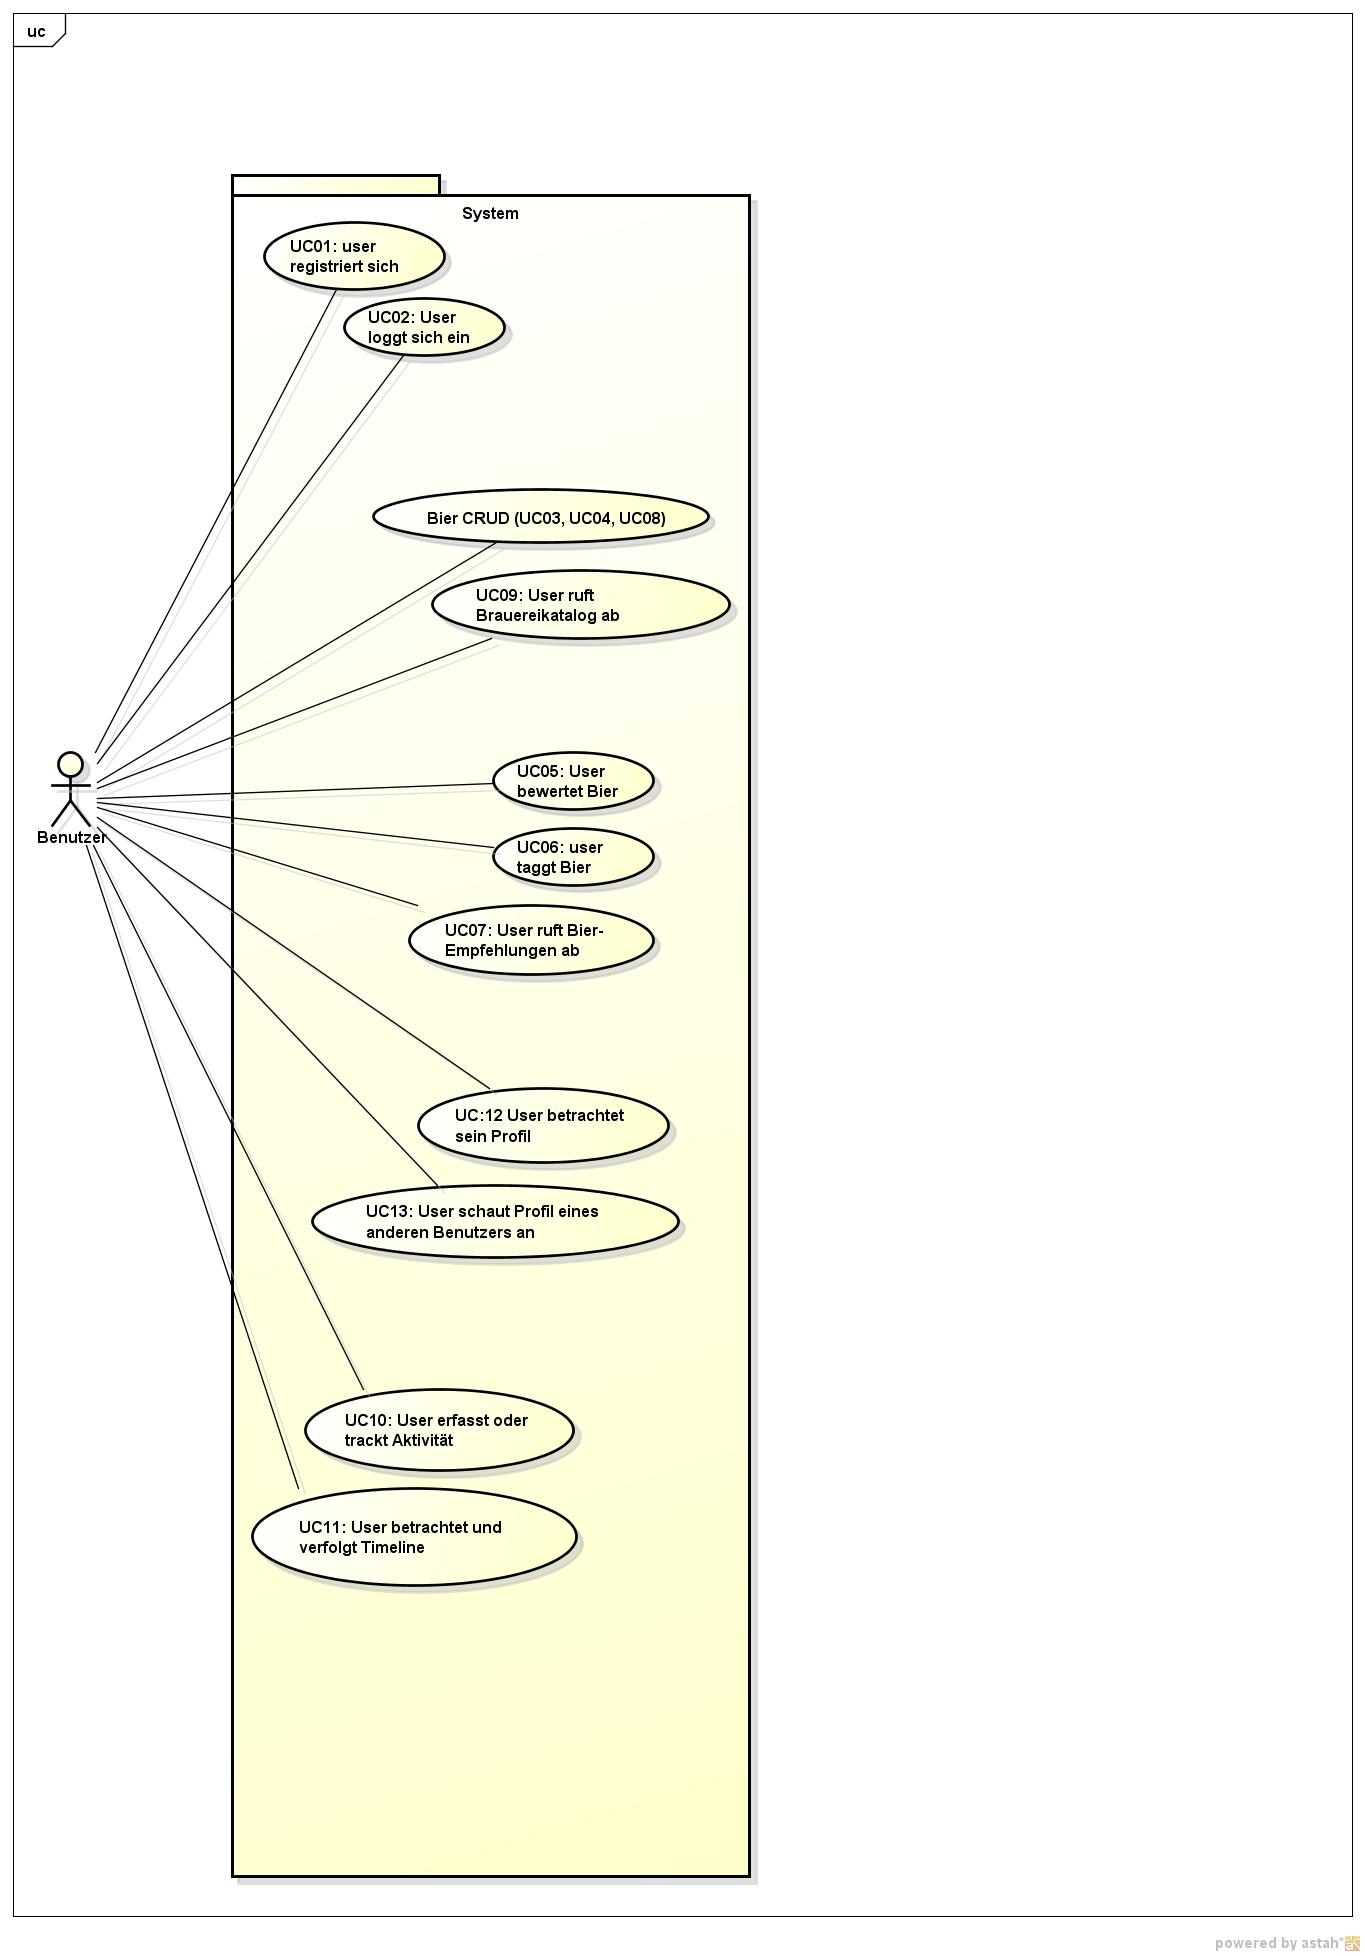
\includegraphics[width=\textwidth]{UseCaseDiagramm.jpg} 
\subsection{Use Cases brief Format}

\subsubsection*{UC01: User registriert sich}
Ein User kann sich registrieren um einen Benutzerzugang (Benutzername, Passwort) zu erhalten. Der Benutzer erhält eine Bestätigungs-Email für die Registration. Er wird nach der Registration automatisch eingeloggt und kann bereits seinen Bierkonsum tracken. Erst wenn er die Email-Adresse per Link bestätigt hat, kann er auch neue Biere erfassen und ändern.
\subsubsection*{UC02: User loggt sich ein}
Ein User kann sich mittels Kombination von Benutzernamen und Passwort am System anmelden.
Der Benutzer hat die Möglichkeit seine Anmeldeinformationen zu speichern, sodass er Sie nicht jedes Mal erneut eingeben muss.
\subsubsection*{UC03: User erfasst ein Bier}
Ein User kann ein neues Bier mit definierten Attributen in das System einpflegen.
\subsubsection*{UC04: User bearbeitet erfasstes Bier}
Ein Benutzer kann die Attribute eines im System erfassten Bieres anpassen und abspeichern.
\subsubsection*{UC05: User bewertet Bier}
Der Benutzer kann ein Bier auswählen und mit einer persönlichen Bewertung versehen. Wenn der Benutzer bereits eine Bewertung erfasst hat, wird diese angezeigt und kann angepasst werden. Der User erfasst dadurch eine Bewertungs-Aktivität.
\subsubsection*{UC06: User taggt Bier}
Der Benutzer kann ein Bier auswählen und mit Schlagwörtern "taggen". Das Taggen wird mit technischen Massnahmen unterstützt, beispielsweise durch Vorschläge.
\subsubsection*{UC07: User ruft Bier-Empfehlungen ab}
Der Benutzer kann auf sein Profil bezogene Empfehlungen für ihm bisher unbekannte (unbewertete) Biersorten abrufen.
\subsubsection*{UC08: User ruft Bier-Katalog ab}
Der Benutzer kann den ganzen Katalog an im System erfassten Bieren in listenartiger Übersicht durchsehen. Durch auswählen eines einzelnen Bieres kann er dessen weitere Attribute abrufen.
\subsubsection*{UC09: User ruft Brauerei-Katalog ab}
Der Benutzer kann den ganzen Katalog an im System erfassten Brauereien durchsehen. Durch auswählen einer einzelnen Brauerei kann er deren weitere Attribute abrufen.
\subsubsection*{UC10: User erfasst Konsum}
Der Benutzer kann eine Konsum-Aktivität erfassen. Die dazugehörigen Informationen sind, das konsumierte Bier, der Zeitpunkt und optional der Ort.
\subsubsection*{UC11: User betrachet und verfolgt Timeline}
Der Benutzer kann eine Timeline betrachten. Die Timeline zeigt die letzten eigenen Aktivitäten sowie die der anderer Benutzer.
\subsubsection*{UC12: User schaut sein eigenes Profil (User-Aktivitäten) an}
Der Benutzer kann im System seine erfassten Aktivitäten (Bewertungen, Konsum) anzeigen.
\subsubsection*{UC13: User schaut Profile (User-Aktiviäten) eines anderen Users an}
Der Benutzer kann Profile anderer Benutzer ansehen. Er sieht dadurch Aktivitäten anderer Benutzer.
\subsection{Use Cases fully dressed Format}
Die Fully dressed use Cases sind im Dokument fully.dressed.usecases.pdf beschrieben.
\section{Nichtfunktionale Anforderungen}
Die Nichtfunktionalen Anforderungen wurden im Dokument Supplementary.specification.pdf festgehalten.
\end{document}